\documentclass[11pt]{article}
\usepackage{amsmath}
\usepackage{amssymb}
\usepackage{graphicx}
\usepackage[hidelinks]{hyperref}
\usepackage{bm}
\usepackage{dcolumn}
\usepackage{multirow}
\usepackage{listings}
\usepackage{authblk}

\graphicspath{{../images/}}
\DeclareGraphicsExtensions{.eps,.png}
\DeclareMathOperator{\sech}{sech}
\newcolumntype{d}[1]{D{.}{.}{#1} }
\lstset{
	basicstyle=\footnotesize\ttfamily,
	frame=single,
	columns=fixed,
	breaklines=true
}

\graphicspath{{../images/}}
\renewcommand{\figurename}{Figure}
\newcommand{\figurenames}{Figures}
%\newcommand{\figname}{Figure}
%\newcommand{\fignames}{Figures}
\newcommand{\figname}{Fig.}
\newcommand{\fignames}{Figs.}
\newcommand{\equationname}{Equation}
\newcommand{\equationnames}{Equations}
%\newcommand{\eqnname}{Equation}
%\newcommand{\eqnnames}{Equations}
\newcommand{\eqnname}{Eq.}
\newcommand{\eqnnames}{Eqs.}


\begin{document}

\title{Introduction to the\\Monterey-Newport Parabolic Equation (MNPE)\\Model}
\author[1]{Kevin B. Smith}
\author[2]{Thomas J. Deal}
\affil[1]{Naval Postgraduate School, Monterey, CA}
\affil[2]{Naval Undersea Warfare Center, Newport, RI}
\date{\today}
\maketitle

\begin{abstract}
The Monterey-Newport Parabolic Equation (MNPE) model calculates pressure and acoustic particle velocity for underwater sources in range-dependent oceans using a split-step Fourier method of solving the parabolic wave equation. This document provides an introduction to version 1.0 of the broadband, two-dimensional MNPE model (MNPE2D). It describes the steps required to build the executable from source code, generate the input files, run the model, and read the outputs. It also includes example outputs the user can re-create to verify the model is running correctly on their system.
\end{abstract}

\newpage
\tableofcontents
\newpage
\listoftables
\listoffigures

\section{Introduction}

In the early 1990s, a numerical code known as the University of Miami Parabolic Equation (UMPE) Model was documented and made available to the general research community\cite{Smith1993}. This model was based on the split-step Fourier (SSF) technique\cite{Hardin1973}, and had been adapted from previous versions developed by Fred Tappert at the University of Miami. A subsequent version, known as the Monterey-Miami Parabolic Equation (MMPE) Model, was developed in the mid 1990s that was more streamlined and user-friendly. This code was thoroughly tested against several existing benchmark scenarios and was found to perform reasonably well during the Shallow Water Acoustic Modeling Workshop help in Monterey, CA in 1999 (SWAM'99)\cite{Smith2001}. Subsequent upgrades to the model included a correction to the treatment of bottom loss\cite{Smith2007}, implementation of the complex density approach to handle shear wave losses\cite{Zhang1995}, and the computation of horizontal and vertical velocity fields\cite{Smith2008}. The latest version of the model, known as the Monterey-Newport Parabolic Equation (MNPE) Model, includes built-in support for a variety of rough ocean surfaces\cite{Tappert} and built-in horizontal and vertical dipole sources, which enable reciprocal vector field calculations\cite{Deal2017}.

This document provides an introduction to version 1.0 of the broadband, two-dimensional MNPE model (MNPE2D). It describes the steps required to build the executable from source code, generate the input files, run the model, and read the outputs. It also includes example outputs the user can re-create to verify the model is running correctly on their system.

\section{Building MNPE}

MNPE is distributed as FORTRAN source code and must be compiled into an executable. The source files are listed in Table~\ref{tab:sourcecode}. In addition to the Fortran source code (*.f), there are two Matlab scripts (*.m) for reading the binary output files. MNPE can be built in Windows, MacOS, or Linux with an appropriate compiler, such as the Intel Fortran Compiler \url{https://software.intel.com/en-us/fortran-compilers} or the GNU Fortran Compiler \url{https://gcc.gnu.org/fortran}. The details of installing and configuring a Fortran development environment are beyond the scope of this document.

\begin{table}[!ht]
	\begin{center}
		\caption{MNPE source code}
		\label{tab:sourcecode}
		\begin{tabular}{c|l}
			\textbf{File} & \textbf{Function} \\
			\hline
			\texttt{Pemp2dbb.f} & Main program \\
    		\texttt{Envprop1.f} & Environment propagator \\
    		\texttt{phsprop.f} & Phase propagator \\
    		\texttt{pesrc.f} & Source generator \\
    		\texttt{Zsgen.f} & Ocean surface generator \\
    		\texttt{fft.f} & Fast Fourier Transform \\
    		\texttt{ssi.f} & Interpolation \\
    		\texttt{peout1.m} & Binary file header reader \\
    		\texttt{peout2.m} & Binary file data reader \\
		\end{tabular}
	\end{center}
\end{table}

Once the development environment is configured, MNPE can be built from the command line as follows:

\begin{table}[!ht]
	\begin{center}
		\caption{Example build commands}
		\label{tab:typeenum}
		\begin{tabular}{c|c|l} 
			\textbf{Platform} & \textbf{Compiler} & \textbf{Command}\\
			\hline
			\multirow{2}{*}{Windows} & Intel & \texttt{ifort *.f /exe:MNPE2D.exe} \\
			& GNU & \texttt{gfortran *.f -o MNPE2D.exe} \\
			\multirow{2}{*}{MacOS/Linux} & Intel &  \texttt{ifort *.f -o MNPE2D}\\
			& GNU & \texttt{gfortran *.f -o MNPE2D} \\
		\end{tabular}
	\end{center}
\end{table}

Alternatively, the user can install CMake \url{https://cmake.org} and use the following \texttt{CMakeLists.txt} file to generate a platform-specific makefile.

\newpage
\lstinputlisting[caption={\texttt{CMakeLists.txt}}]{../../src/CMakeLists.txt}

The executable has no external dependencies and can be run from any directory. The user may want to run the executable from a single location and add that location to their system's \texttt{PATH} variable. Alternatively, the executable can be copied into multiple working directories and run locally in each one.

\section{Description of Input Data}

MNPE reads input data for each run from 8 plain text files. These files must all be in the same directory as each other, but do not need to be in the same directory as the MNPE executable, as long as the executable is on the system \texttt{PATH}. A detailed description of these files follows. Note that when entering numeric values in these files, floating point values must always include a decimal point, even if they are whole numbers. Fortran automatically interprets numbers without a decimal point as integers.

\subsection{Main input file}

The main input file must be named \texttt{pefiles.inp}. All other input files are specified in this file. The placement of the input data in this file MUST follow the ``:'' character in its current position. 

\lstinputlisting[caption={\texttt{pefiles.inp}},label={lst:pefiles}]{../../examples/Monopole/pefiles.inp}

The first several inputs simply define the names of the other input files and are self-explanatory. Note that the output data files (pressure, velocity\_r, velocity\_z) will be binary files and will overwrite any other files by those names. The following line, e.g.
\lstinputlisting[firstline=11,lastline=11,frame=none]{../../examples/Monopole/pefiles.inp}
specifies the ``requested'' number of points in depth, minimum depth [m], and maximum depth [m] to output. The program will try to come as close to this request as possible. Similarly, the next line, e.g.
\lstinputlisting[firstline=12,lastline=12,frame=none]{../../examples/Monopole/pefiles.inp}
specifies the ``requested'' number of points in range, minimum range [km], and maximum range [km] to output. The program will try to come as close to this request as possible. The final line in this file, e.g.
\lstinputlisting[firstline=13,lastline=13,frame=none]{../../examples/Monopole/pefiles.inp}
is designed to allow flexibility. These numbers represent the vertical FFT size (INTEGER multiple of 2), the range step [km], the maximum depth of calculation [m], and the reference sound speed [m/s]. All of these numbers can be set to 0 and default values will be chosen based on the other input data. The only exception to this is c0 which will always be chosen as 1500 m/s unless otherwise stated. Note that the default values for range step and FFT size are chosen to produce the most accurate result, not the most efficient. You may find adequate accuracy with larger range steps or smaller FFT sizes which would speed up your run times (important for very high frequency or very broadband calculations).

\subsection{Source data}

All of the source information is contained in the file \texttt{pesrc.inp}. Again, the format of this file must be maintained insomuch as the actual values must follow the ``:'' character in its current position. The description preceding each value makes this file mostly self-explanatory. 

\lstinputlisting[caption={\texttt{pesrc.inp}}]{../../examples/Monopole/pesrc.inp}

Note that four source types are available - a vertical line array (approximated by a continuous line array) and three wide-angle sources that approximate a monopole, horizontal dipole, and vertical dipole point source. If a positive array length is specified, a simple line array is modeled by a sinc function. The D/E angle is then used to steer the main beam of the array, positive angles steering the beam downward, positive angles steering the beam upward. The different point sources are identified by zero or negative values, as shown in Table~\ref{tab:sourcetypes}. Since this is a 2D version of MNPE, the horizontal dipole is aligned in the radial direction. When a point source is specified, the D/E angle input is ignored. All numbers in this file are FLOATS with the exception of the last value, the number of frequencies (must be a power of two), which must be an integer.

\begin{table}[!ht]
	\begin{center}
		\caption{Array length codes for monopole and dipole point sources}
		\label{tab:sourcetypes}
		\begin{tabular}{d{1}|l} 
			\textbf{Value} & \multicolumn{1}{c}{\textbf{Description}}\\
			\hline
			>0.0 & Vertical Uniform Linear Array \\
			0.0 & Monopole Source \\
			-1.0 & Horizontal Dipole Source \\
			-2.0 & Vertical Dipole Source \\
		\end{tabular}
	\end{center}
\end{table}

Additional details on the implementation of the two dipole source types in MNPE can be found in Appendix~\ref{app:dipolesource}.

\subsection{Sound speed profile data}

The sound speed profile data is contained in \texttt{pessp.inp}. It has the ability to hold multiple profiles taken at multiple ranges and defined as a function of depth. The first line contains a single Boolean value (0 or 1) to define whether or not water volume attenuation should be used (no or yes). The second line contains a single number indicating the number (INTEGER) of sound speed profiles contained in the first radial. The following line contains two numbers indicating the range [km] (FLOAT) of the current profile and the number (INTEGER) of sound speed values in depth at this range. Finally, the profile itself is defined by a pair of numbers (FLOATS) stating the depth [m] and sound speed [m/s] of the sound speed profile. For isovelocity profiles, only a single data pair (depth, sound speed) is required at each range.

\lstinputlisting[caption={\texttt{pessp.inp}}]{../../examples/Monopole/pessp.inp}

\subsection{Rough ocean surface data}\label{sec:roughsurface}

Rough ocean surface data is contained in \texttt{pesurf.inp}. The first line has a single number (INTEGER) that specifies the surface spectrum type, as shown in Table~\ref{tab:surfaces}. 

\begin{table}[!ht]
	\begin{center}
		\caption{Surface spectrum type enumerations}
		\label{tab:surfaces}
		\begin{tabular}{c|l} 
			\textbf{Value} & \textbf{Description}\\
			\hline
			0 & Flat Surface \\
			1 & RMS Roughness and Correlation Length \\
			2 & Pierson-Moskowitz \\
			3 & JONSWAP \\
			4 & User-Defined \\
		\end{tabular}
	\end{center}
\end{table}

The second line contains a single number (FLOAT) that is the tide height [m] referenced to the mean lower low water level (MLLW). This number is measured positive up, as is reported by tide gauges. If a flat surface is selected, there is no additional information in the file. For all other spectrum types, the third line in the file has three numbers (INTEGER followed by a FLOAT and another INTEGER). The first number is used to set the random seed. Each seed produces a repeatable random number sequence, so this parameter should be varied if a different surface realization is desired each time MNPE runs. The second number is the time in seconds since the initial surface realization. When the goal is to compute many different realizations and average the result, the seed should be changed for each run and the time should be held constant. When the goal is to evolve a surface over time, the seed should be held constant for each run and the time should be varied. The third number sets the wave propagation direction. For waves arriving from the $+r$ direction (going toward the source at $r=0$), enter a positive value, and for waves arriving from the $-r$ direction (going away from the source at $r=0$), enter a negative value. For standing waves, enter 0.

The following lines are different for the different spectrum types. For the Pierson-Moskowitz spectrum\cite{PM}, line four contains a single number (FLOAT) equal to the wind speed [m/s] at a height of 19.5 meters above the sea surface. For the JONSWAP spectrum\cite{JONSWAP}, line four contains two numbers (FLOATS). The first is the wind speed [m/s] at a height of 10 meters above the sea surface, and the second is the fetch [m]. Finally, for the user-defined spectrum, the fourth line contains a single number (INTEGER) indicating the number of points $N_{SPEC}$ in the user-specified spectrum. ZSGEN will then read the following $N_{SPEC}$ lines from the file, with each line containing two numbers (FLOATS): the frequency [Hz] and the spectral density [m$^2$/Hz]. These frequency/spectrum pairs are for a single-sided magnitude spectrum, so all frequencies and spectral densities are positive. The frequency sampling interval does not need to be constant, because these values are resampled internally by ZSGEN to match the realization length and FFT size. Example surface spectrum files are included with the source code. An example using the JONSWAP spectrum is shown below.

\newpage
\lstinputlisting[caption={\texttt{pesurf.inp}}]{../../examples/RoughSurface/pesurfjonswap.inp}

Additional details on acquiring measured surface wave spectra and the implementation of user-defined rough ocean surfaces in MNPE are contained in Appendix~\ref{app:roughsurface}.

\subsection{Bathymetry and bottom properties data}

The bathymetry at the water/bottom interface is contained in \texttt{pebath.inp}. The first line contains the number (INTEGER) of bathymetry points defined. This is then followed by the bathymetry defined by pairs of numbers (FLOATS) stating the range [km] and depth [m] or the bathymetry point. The range points in the bathymetry file are not required to coincide with range points in the sound speed profile file. For flat bottoms, only a single data pair (range, depth) is required.

\lstinputlisting[caption={\texttt{pebath.inp}}]{../../examples/Monopole/pebath.inp}

This acoustic parameters of the medium just below the water/bottom interface are contained in \texttt{pebotprop.inp}. Note that bottom properties are not depth dependent (with the exception of the sound speed which can have a constant gradient) but can be range-dependent. This range dependency can be entirely independent of the bathymetry. In other words, the ranges specifying changes in the bottom properties do no have to coincide with the ranges specifying changes in the bathymetry. Therefore, the first line contains the number (INTEGER) of different range points at which the bottom properties are defined. This is then followed by that many lines, each line containing seven numbers (FLOATS): range [km] where these values apply, sound speed [m/s], sound speed gradient [1/s], density [g/cm$^3$], compressional attenuation [dB/m/kHz], shear speed [m/s], and shear attenuation [dB/m/kHz].

\lstinputlisting[caption={\texttt{pebotprop.inp}}]{../../examples/Monopole/pebotprop.inp}

\subsection{Deep bathymetry and bottom properties data}

The data for a second, ``deep,'' bathymetry layer below the water/sediment interface is contained in \texttt{pedbath.inp}. The bathymetry values are measured relative from the sea surface. Therefore, an extremely deep bathymetry value (deeper than the computational depth) will not even be used whereas a bathymetry value shallower than the water/bottom depth will supercede the upper layer and become the water/bottom depth (e.g., as would occur for a rock outcrop in a sediment pool). This file has the same format as the upper layer bathymetry file, \texttt{pebath.inp}. The acoustic parameters of the deep bathymetry layer are contained in \texttt{pedbotprop.inp}. Its format is identical to the format of the bottom properties file described above. Examples of these two files are listed below.

\lstinputlisting[caption={\texttt{pedbath.inp}}]{../../examples/Monopole/pedbath.inp}

\lstinputlisting[caption={\texttt{pedbotprop.inp}},label={lst:pedbotprop}]{../../examples/Monopole/pedbotprop.inp}

\section{Running MNPE}

MNPE runs from the command line. The current working directory must contain the 8 \texttt{*.inp} files. Since reading the output requires the use of Matlab scripts \texttt{peout1.m} and \texttt{peout2.m}, it is convenient to execute MNPE from Matlab also. This can be done with \texttt{system('MNPE2D')}, if the MNPE executable is on the user's system \texttt{PATH}. To execute a local copy of the executable use \texttt{system('./MNPE2D')}.

While MNPE runs, it prints updates to the command line to indicate progress to the user. It processes each frequency sequentially, printing the current frequency followed by periodic range updates. An example is shown in Listing~\ref{lst:runoutput}.

\lstinputlisting[firstline=7,caption={MNPE command line output},label={lst:runoutput}]{../images/RunOutput.txt}

Running MNPE generates binary output files \texttt{press.bin}, \texttt{apvr.bin}, and \texttt{apvz.bin}. To read and plot the outputs, run \texttt{peout1} and \texttt{peout2} from the Matlab command prompt. The scripts can either be copied into the MNPE working directory and run from there, or they can be saved in a directory that is included in the Matlab \texttt{PATH}.

The first script to run is \texttt{peout1}, which reads header data from the binary files. The script will prompt the user for the name of the file to be read. After the file name is entered by the user, the script loads that data into the Matlab workspace and displays information from the file header, as shown in Listing~\ref{lst:peout1output}. The header includes information about the run, including the actual sampling used in depth and range. These may differ from the ``requested'' values in \texttt{pefiles.inp}.

\lstinputlisting[firstline=3,caption={\texttt{peout1} output for \texttt{press.bin}},label={lst:peout1output}]{../images/peout1Output.txt}

After reading the header, the field data can be extracted by running \texttt{peout2}. It will prompt the user with multiple options, as shown in Table~\ref{tab:peout2options}.

\begin{table}[!ht]
	\begin{center}
		\caption{Options available for \texttt{peout2}}
		\label{tab:peout2options}
		\begin{tabular}{c|l} 
			\textbf{Option} & \textbf{Description}\\
			\hline
			1 & Starting field data \\
			2 & Data for single radial \\
			3 & Data for single range \\
			4 & Data for single depth \\
			5 & Data for single interface \\
			6 & Travel time data \\
		\end{tabular}
	\end{center}
\end{table}

Option 1 outputs the starting field as a function of depth and frequency in the variable \texttt{psi0}. Option 2 outputs the field as a function of depth and range in the variable \texttt{press}. The user is prompted to select a single frequency when data for multiple frequencies was calculated. The variable name \texttt{press} is used for velocity data as well as pressure data, so the user must rename this variable to prevent subsequent calls to \texttt{peout} from overwriting it. Option 3 prompts the user for a single range and outputs field data as a function of depth and frequency for that range in \texttt{press}. Similarly, Option 4 prompts the user for a single depth and outputs field data as a function of range and frequency for that depth in \texttt{pressd}. When the user selects option 5, \texttt{peout2} prompts the user to select either the water/bottom interface or bottom/deep bottom interface and then outputs the field at that interface's depth as a function of range and frequency in \texttt{pressd}. Unlike option 4, option 5 follows the bathymetry in a range-dependent environment. 

Option 6 can be used when the source input file specifies multiple frequencies.  The processing assumes a power of 2 number of frequencies
$N_f$, and defaults to a Hanning source amplitude spectrum across the bandwidth $BW$.  The user must ensure that the frequency sampling, defined by $BW/(N_f-1)$, is sufficient to avoid wrap-around of the travel time results.

Within option 6, there are multiple sub-options.  Sub-option 6.1 computes the broadband travel time data along a single radial at a specified range. Furthermore, within this sub-option, one can choose between simply producing a plot of time vs. depth, or producing a plot of time vs. vertical arrival angle, as could be processed by a vertical array through standard wavenumber processing techniques.  This latter option will also ask the user to define the upper and lower depths of the vertical array to process beams. Sub-option 6.2 computes the broadband travel time data at a single depth. The subsequent plot displays travel time vs.range. Sub-option 6.3 is similar to 6.2, but computes the broadband travel time data at an interface.

After generating plots, the user is prompted with the option to save the data to a \texttt{.mat} file. The output data remains in the current Matlab workspace even if the user does not save it to a \texttt{.mat} file. A selection of commonly-used workspace variables is listed in Table~\ref{tab:peoutdata}.

\begin{table}[!ht]
	\begin{center}
		\caption{Selected workspace variables generated by \texttt{peout1} and \texttt{peout2}}
		\label{tab:peoutdata}
		\begin{tabular}{c|l} 
			\textbf{Name} & \textbf{Description}\\
			\hline
			\texttt{nf} & Number of frequencies \\
			\texttt{nrout} & Number of points in range vector \\
			\texttt{nzout} & Number of points in depth vector \\
			\texttt{freq} & Frequency vector [Hz] (1 x \texttt{nf})\\
			\texttt{freqout} & Frequency selected by user [Hz] \\
			\texttt{rngout} & Range selected by user [km] \\
			\texttt{depout} & Depth selected by user [m] \\
			\texttt{rng} & Range vector [km] (\texttt{nrout}  x 1)\\
			\texttt{dep} & Depth vector [m] (1 x \texttt{nzout})\\
			\texttt{surf} & Ocean surface vector [m] (\texttt{nrout}  x 1)\\
			\texttt{bath} & Bathymetry vector [m] (\texttt{nrout}  x 1)\\
			\texttt{dbath} & Deep bathymetry vector [m] (\texttt{nrout}  x 1)\\
			\texttt{press} & Complex transmission loss data \\
		\end{tabular}
	\end{center}
\end{table}

\subsection{Example outputs}

The following examples are included with the MNPE distribution to demonstrate the basic features and usage of MNPE. The user is encouraged to recreate these plots with their MNPE application to verify their application is working as intended. Note that in these plots, the color scale has been changed from the default values.

\subsubsection{Flat}

The Flat environment is a 200 m deep waveguide of constant depth, with a constant sound speed of 1500 m/s. The fluid bottom has sound speed 1700 m/s, density 1.5 g/cm$^3$, and attenuation 0.333 dB/m/kHz. There is no deep bottom. The source is at a depth of 100 m, producing a single tone at 200 Hz.

\begin{figure}[!ht]
\begin{center}
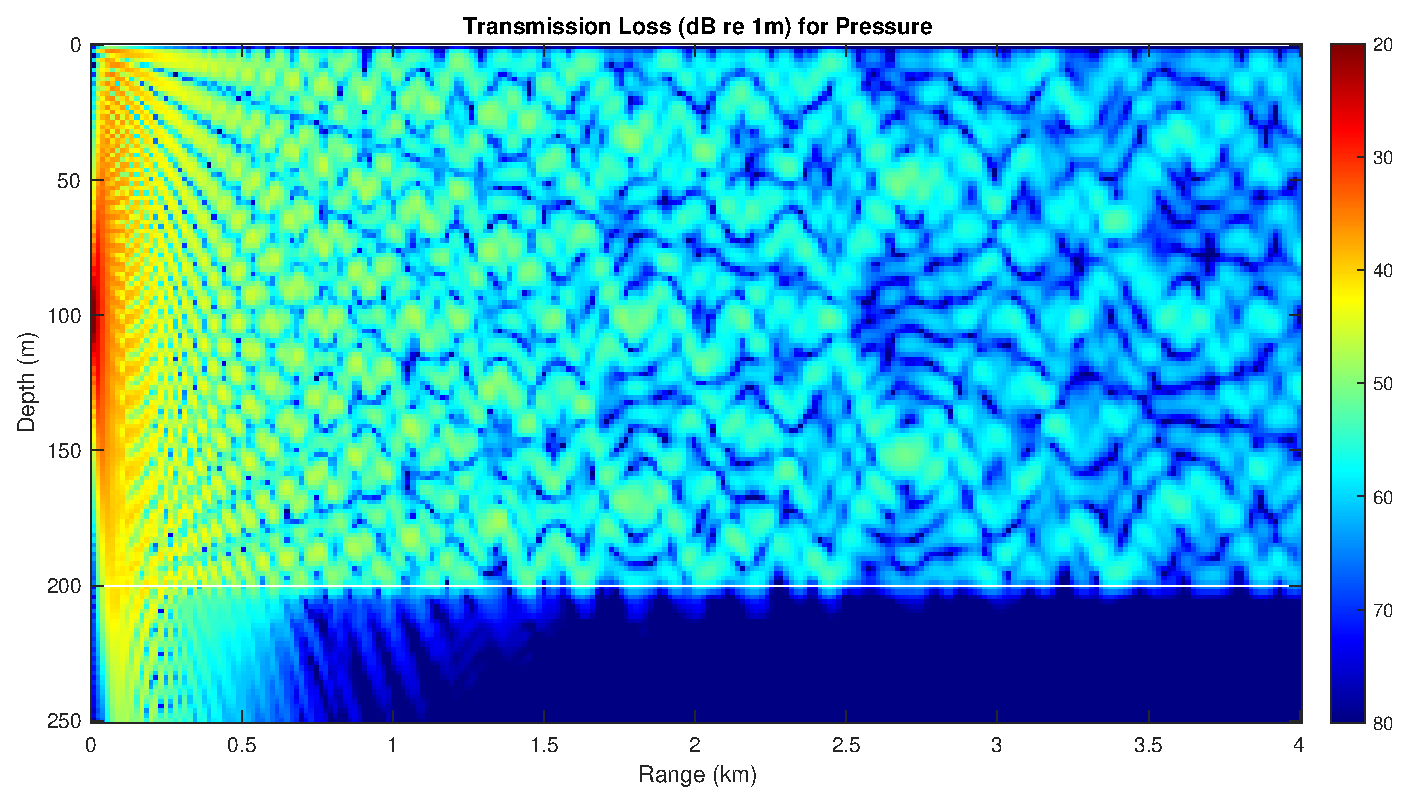
\includegraphics[width=\textwidth]{FlatP.eps}
\caption{\label{fig:FlatP}Flat environment pressure transmission loss}
\end{center}
\end{figure}

\clearpage
\subsubsection{ASA Wedge}

The ASA Wedge environment is identical to the Flat environment, except that the bathymetry varies linearly from 200 m at range 0 km to 0 m at range 4 km. The source is again at a depth of 100 m, producing a single tone at 200 Hz.

\begin{figure}[!ht]
\begin{center}
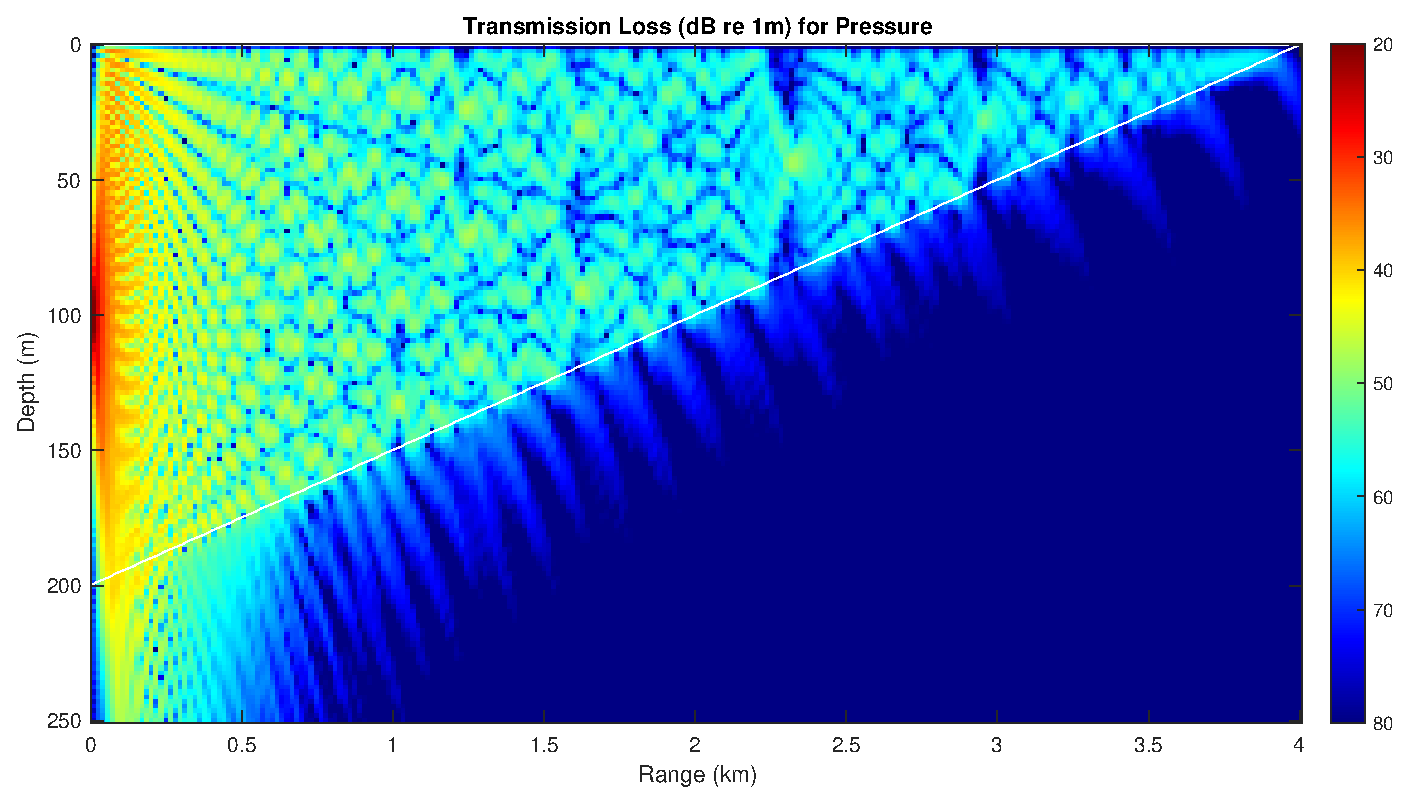
\includegraphics[width=\textwidth]{ASAWedgeP.eps}
\caption{\label{fig:ASAWedgeP}ASA Wedge environment pressure transmission loss}
\end{center}
\end{figure}

\clearpage
\subsubsection{Monopole Source}

This example demonstrates pressure and vertical velocity outputs for a monopole source in the Flat environment with 100 m bathymetry. The source is at a depth of 50 m, producing a single tone at 60 Hz.
 
\begin{figure}[!ht]
\begin{center}
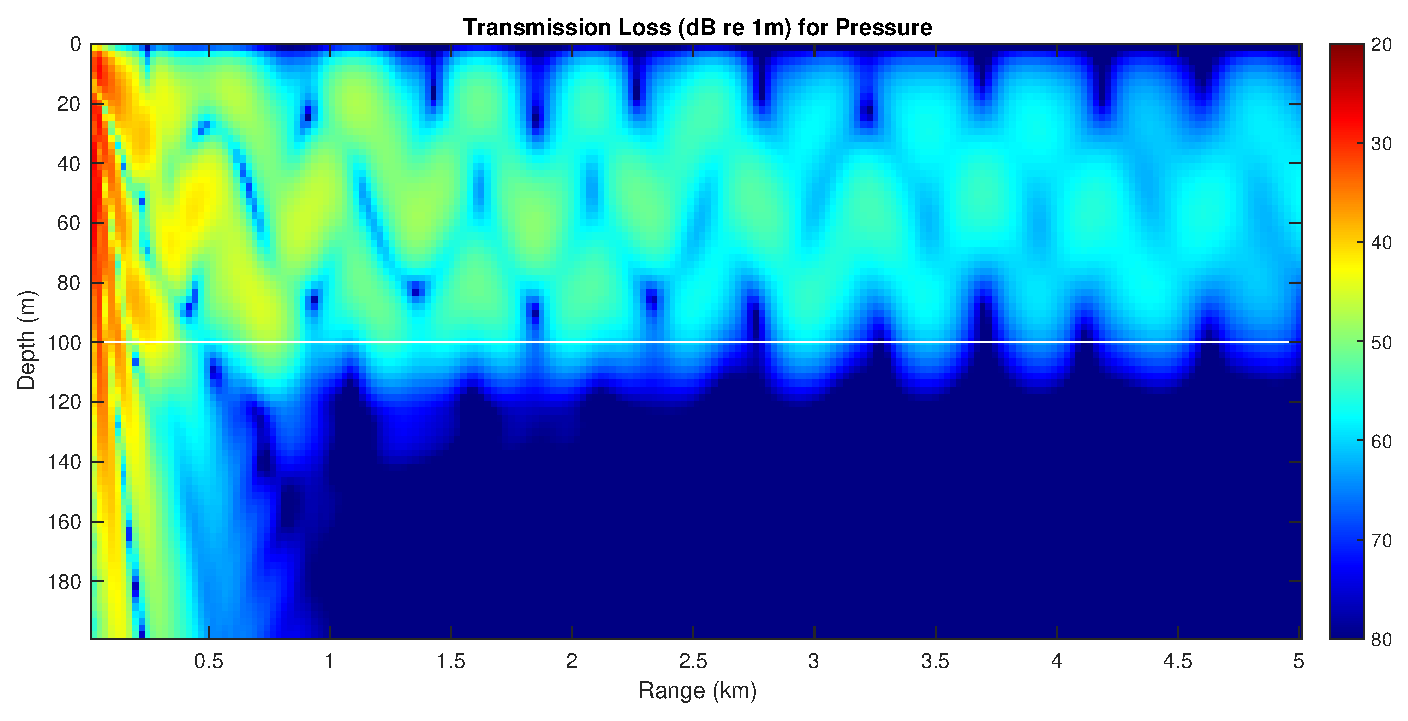
\includegraphics[width=\textwidth]{MonopoleP.eps}
\caption{\label{fig:MonopoleP}Monopole Source pressure transmission loss}
\end{center}
\end{figure}

\begin{figure}[!ht]
\begin{center}
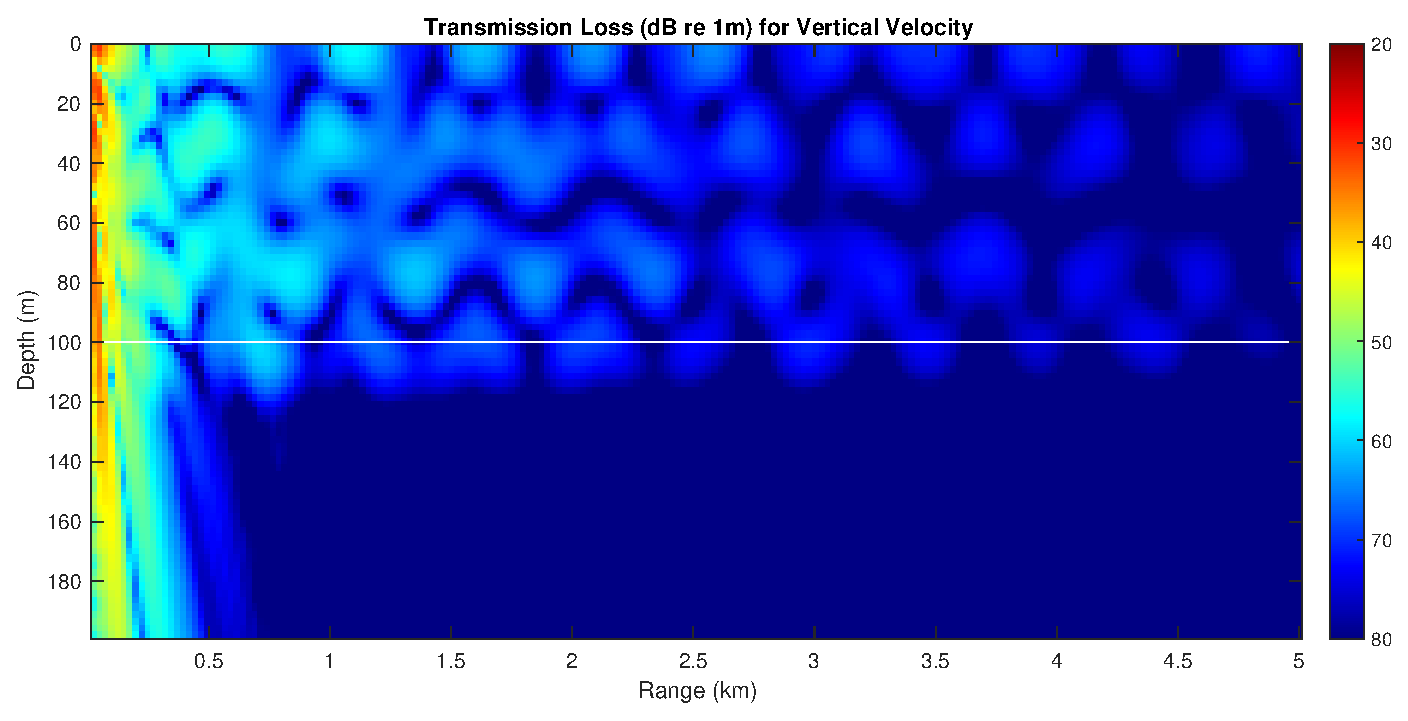
\includegraphics[width=\textwidth]{MonopoleVZ.eps}
\caption{\label{fig:MonopoleVZ}Monopole Source vertical velocity transmission loss}
\end{center}
\end{figure}

\clearpage
\subsubsection{Vertical Dipole Source}

This example demonstrates pressure and vertical velocity outputs for a vertical dipole source. It is identical to the Monopole example, except the source has been replaced with a vertical dipole.

\begin{figure}[!ht]
\begin{center}
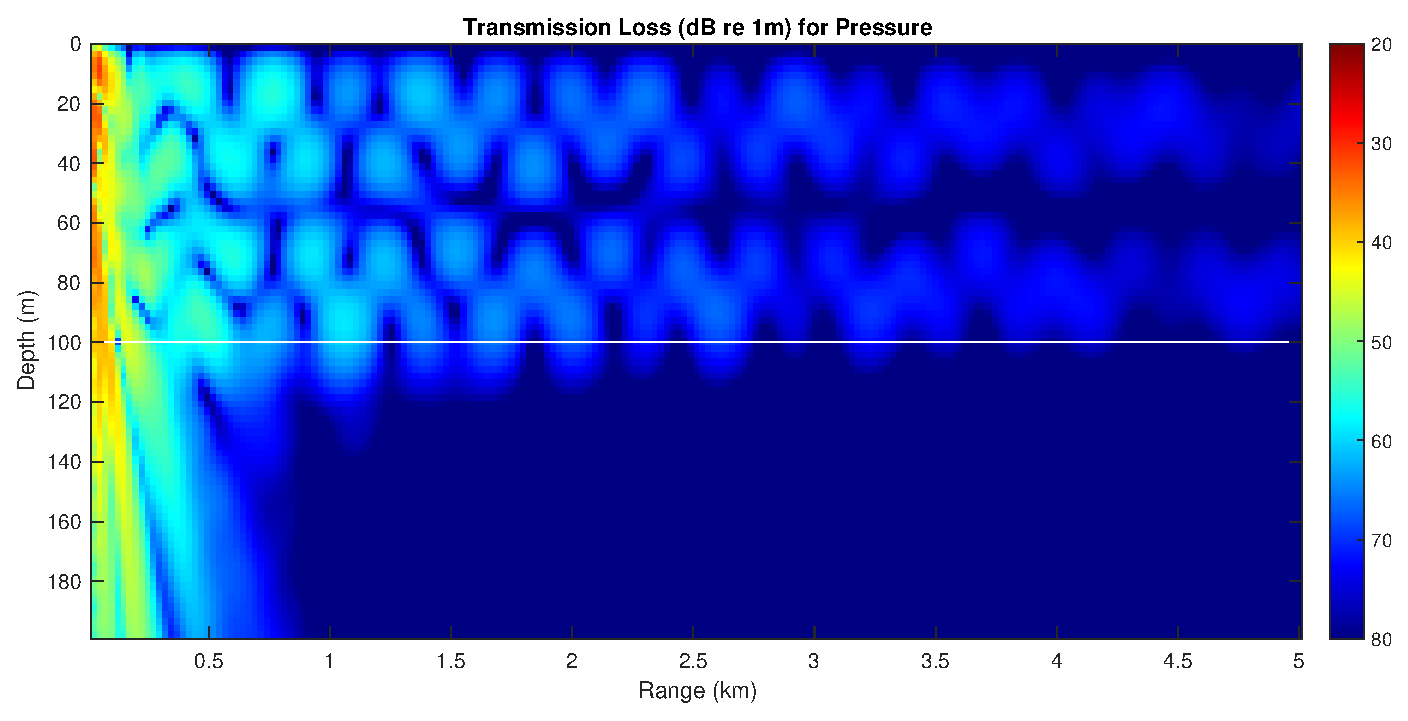
\includegraphics[width=\textwidth]{DipoleP.eps}
\caption{\label{fig:DipoleP}Vertical Dipole Source pressure transmission loss}
\end{center}
\end{figure}

\begin{figure}[!ht]
\begin{center}
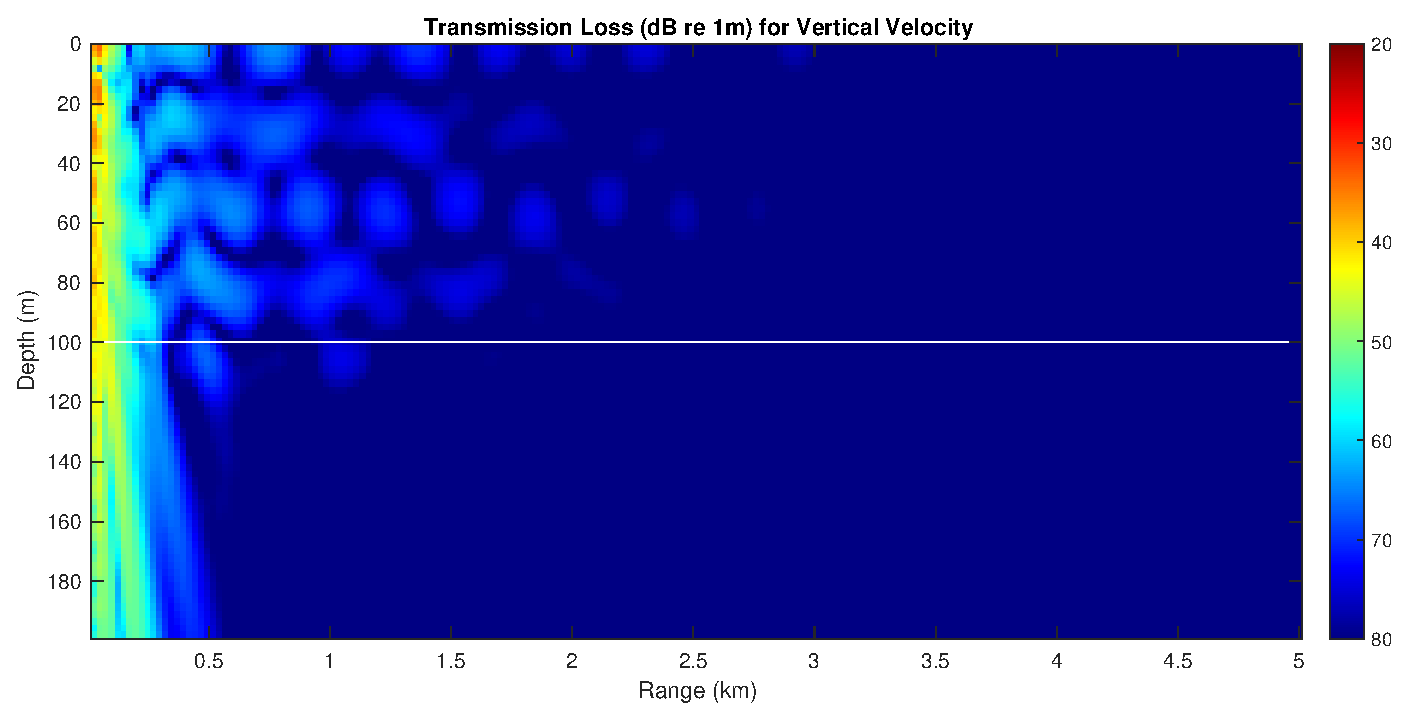
\includegraphics[width=\textwidth]{DipoleVZ.eps}
\caption{\label{fig:DipoleVZ}Vertical Dipole Source vertical velocity transmission loss}
\end{center}
\end{figure}

\clearpage
\subsubsection{Rough Surface}

This example demonstrates the effects of a rough ocean surface. It repeats the Flat environment example with a Pierson-Moskowitz surface wave spectrum for 20 m/s wind speed.

\begin{figure}[!ht]
\begin{center}
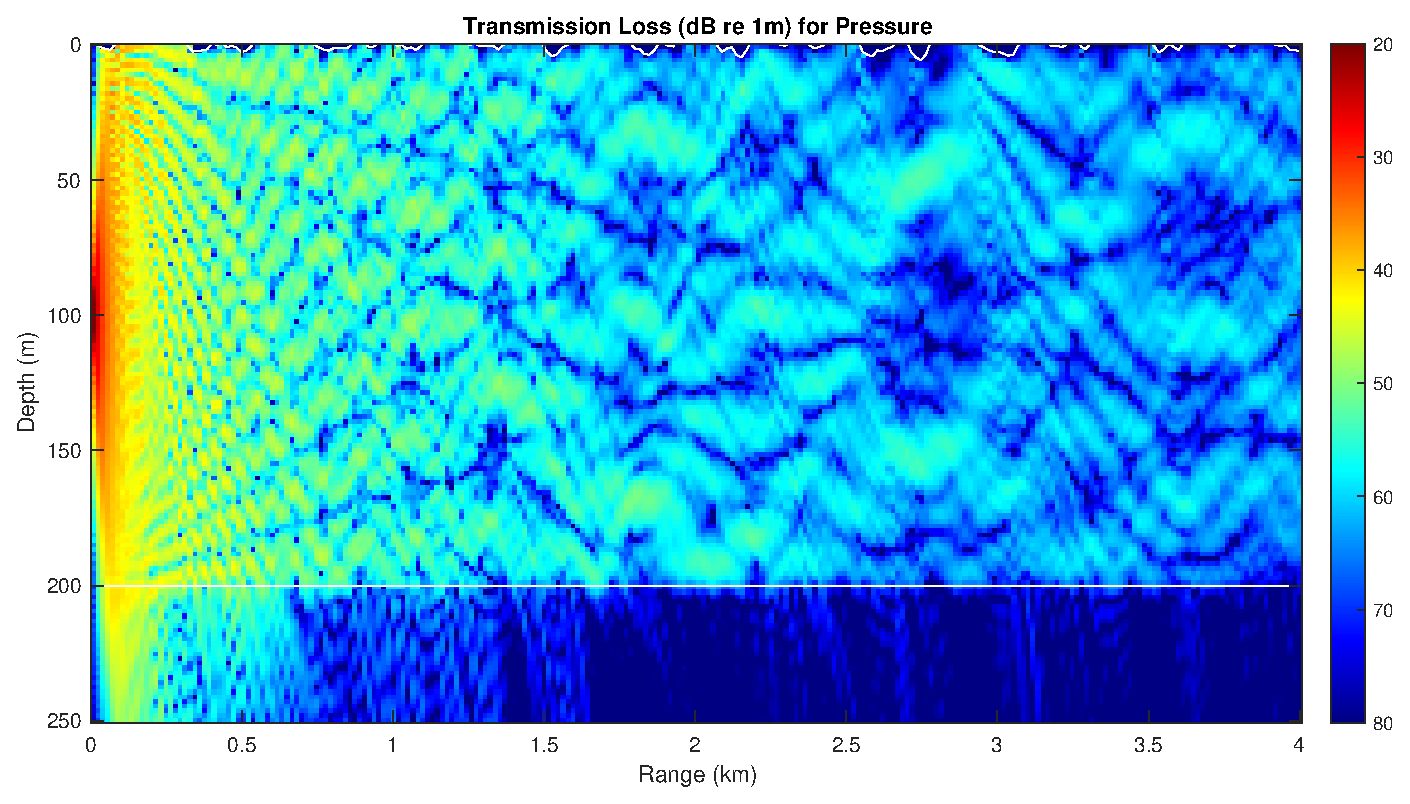
\includegraphics[width=\textwidth]{RoughSurfaceP.eps}
\caption{\label{fig:RoughSurfaceP}Flat environment with rough surface pressure transmission loss}
\end{center}
\end{figure}

\clearpage
\subsubsection{Travel Time}

The travel time example uses the Flat environment, but the source is now broadband. Its center frequency is 500 Hz, with 256 frequencies spanning a bandwidth of 255 Hz. The plot is for a range of 1 km.

\begin{figure}[!ht]
\begin{center}
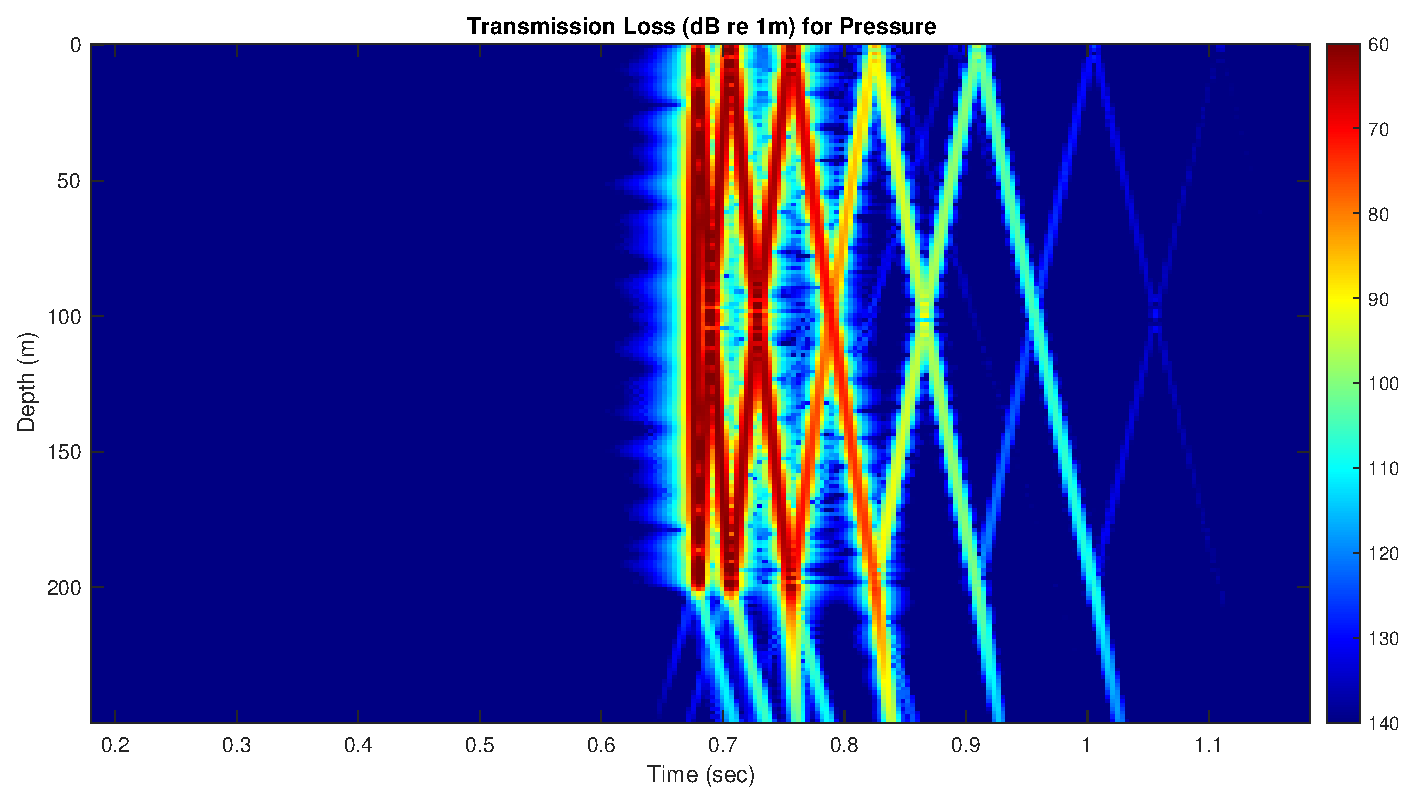
\includegraphics[width=\textwidth]{TravelTimeP.eps}
\caption{\label{fig:TravelTimeP}Flat environment pressure travel time}
\end{center}
\end{figure}


\appendix 
\renewcommand\thefigure{\thesection.\arabic{figure}}  
\renewcommand\theequation{\thesection.\arabic{equation}}  
\numberwithin{equation}{section}

\section{Dipole Sources in MNPE}\label{app:dipolesource}

Generating fields for dipole sources is accomplished by modifying the PE starter field. Vecherin, et al.\cite{Vecherin2011} prescribes an equivalent source method that decomposes vertical and horizontal dipole sources into vertical monopole arrays with element amplitude scaling such that the array source strength is equal to that of a single monopole.

A vertical dipole is a special case of a vertical array with two elements 180 degrees out of phase with each other and separated by a distance $2d_z$ much smaller than a wavelength ($kd_z\leq0.1$). The desired shape of the acoustic field for this source is $\cos(\phi)$ for angles $\phi$ measured from the vertical axis. The horizontal dipole has a desired shape of $\sin(\phi)$, which Vecherin represents as a sum of cosines for angles close to $\pi/2$,
\begin{equation}
\sin(\phi) \approx 1 - \frac{1}{2}\cos^2(\phi) - \frac{1}{8}\cos^4(\phi),\label{eq:sineapprox}
\end{equation}
which is valid for wide-angle PE calculations. The $\cos^n(\phi)$ terms in \eqnname~(\ref{eq:sineapprox}) can be represented by arrays of 1, 3, and 5 elements vertically spaced by $2d_z$, which when added together produce the desired PE starter field. Although these amplitude weights and element spacings can be implemented with MNPE's existing vertical array source, the utility of dedicated horizontal and vertical dipole sources led to a direct implementation of the starter field in the vertical wavenumber domain such that the user need only specify the source depth and frequency.

Each of these point sources is implemented with an analytic starter, which accounts for reflection from a pressure release surface. The analytic starter does not account for reflection from the sea floor, which can be important in shallow water or when the source is close to the bottom. The dipole starters are further limited by the vertical extent of their equivalent arrays: when the source is located near the surface or bottom, some array elements may be on the other side of the boundary, and they do not produce the correct acoustic fields. These errors are more pronounced for sources near the surface than for sources near the bottom, since the depth mixing function at the bottom boundary introduces a smoother transition than the perfectly reflecting ocean surface. A modal starter may be more appropriate for dipole sources near surface and bottom boundaries in some cases.

\section{1D Rough Ocean Surface Modeling in MNPE}\label{app:roughsurface}

\subsection{Obtaining real-time surface wave spectra}

The National Data Buoy Center (NDBC - \url{http://www.ndbc.noaa.gov}) provides online access to data from a variety of data collecting buoys and coastal stations, including waverider buoys that record wave height. One example is Station 46239 located approximately 10 nautical miles west of the Point Sur Lighthouse at $36^\circ 20'28''$ N, $122^\circ 6'6''$ W in 369 meters of water. This is a Datawell directional buoy Mark 3 operated by Scripps Institution of Oceanography.

The NDBC site provides real-time spectral summary data and raw spectral data recorded at 30-minute intervals for the previous 45 days. The summary data includes calculations of significant wave height, period, and direction. It also provides these calculations separately for swell and wind-driven waves by partitioning the spectra into low- and high-frequency regions. This summary data can be used to calculate an equivalent Pierson-Moskowitz\cite{PM} or JONSWAP\cite{JONSWAP} spectrum by relating sea state and wind speed to significant wave height with empirical formulas\cite{Hodges}.

The raw spectral data provides a higher resolution alternative to these empirical spectra formulas. This data is also reported at 30-minute intervals for the last 45 hours and consists of wave spectral energy density $S(f)$ in m$^2$/Hz versus frequency $f$. The frequency vector is not uniformly sampled but instead uses 5 mHz sampling from 25 mHz to 100 mHz and 10 mHz sampling from 110 mHz to 580 mHz.

Both the summary and raw spectra files can be retrieved from the NDBC website via http access and saved as delimited text files. This raw data can be copied directly into \texttt{pesurf.inp} without further processing, as described in Section~\ref{sec:roughsurface}. The next section describes how MNPE generates a realization of a rough surface with the same statistical parameters as the requested surface spectrum.

\newpage
\subsection{Generating wave surface realizations}

Once a wave energy density spectrum has been obtained, some care must be taken when using it to generate a realization of a sea surface to account for energy conservation and to avoid sampling issues\cite{Mobley}. This section describes those steps, which are the same for Pierson-Moskowitz, JONSWAP, and user-defined spectra.

\subsubsection{Domain size and sampling}

The first task is to determine the required domain size $L$ and sampling $dx$. These parameters are linked to the number of samples used to compute the spatial FFT, $N_{FFT}$, but there is some flexibility in choosing them. The goal is to have a surface height defined on every range grid used by MNPE up to the maximum computation range. Therefore, a natural choice is to let $dx$ equal the range sampling and $L$ equal the maximum range. In this case, $N_{FFT}=L/dx$ is not guaranteed to be an even power of 2, which could be a problem for the FFT routine already in MNPE. The solution is to zero-pad the spectrum such that $N_{FFT}$ equals the next power of 2 greater than $L/dx$. If the surface realization is to be computed outside MNPE, FFT implementations such as that found in Matlab automatically handle any value for $N_{FFT}$.

An alternative option is to set a fixed power of two for $N_{FFT}$ and $dx$ and generate a wave profile up to range $L=N_{FFT}*dx$. If $L$ is greater than the maximum computational range, the profile can be truncated. If $L$ is less than the maximum computational range, the profile can be repeated every $L$ meters. Since it will be produced by Fourier synthesis there will be no discontinuities at the boundaries.

Whatever method is used to choose the spatial sampling parameters, they must be checked against the wavenumber sampling to ensure there is sufficient resolution in the wavenumber domain to capture the spectrum characteristics. The wavenumber sampling interval $dk=2\pi/L$, so $L$ must be chosen large enough that $dk$ adequately samples the wave spectrum.

\subsubsection{Conversion to spatial spectrum}

Once sampling has been determined, we need to convert the spectrum to the wavenumber domain. The Pierson-Moskowitz and JONSWAP spectra are stated in terms of radial frequency $\omega=2\pi f$, and the spectra recorded by NDBC are stated in terms of frequency $f$, but to generate a spatial wave profile we need the magnitude spectrum stated in terms of spatial frequency or wavenumber $k$. The conversion from frequency to wavenumber takes the form
\begin{equation}
S(k) = S(f)\frac{\partial f}{\partial k}.\label{eq:Sconvert}
\end{equation}

The relationship between frequency and wavenumber for surface gravity waves depends on the dispersion relationship\cite{Hodges}
\begin{equation}
f(k,H) = \frac{1}{2\pi}\sqrt{gk\tanh(kH)},\label{eq:Dispersion}
\end{equation}
where $g$ is the gravitational acceleration constant and $H$ is the water depth. This equation is often simplified into a ``deep-water'' version for $kH\gg 1$,
\begin{equation}
f(k) = \frac{1}{2\pi}\sqrt{gk},
\end{equation}
which is non-dispersive and a ``shallow-water'' version for $kH\ll 1$, 
\begin{equation}
f(k,H) = \frac{k}{2\pi}\sqrt{gH},
\end{equation}
which is dispersive. We will use the full equation for maximum flexibility in shallow, deep, and intermediate water depths. The derivative required for \eqnname~(\ref{eq:Sconvert}) is
\begin{equation}
\frac{\partial f(k,H)}{\partial k} = \frac{g\tanh(kH) + gkH\sech^2(kH)}{4\pi\sqrt{gk\tanh(kH)}}.
\end{equation}

Since the NDBC data is sampled with nonuniform frequency spacing, we must resample the spectrum over the uniformly-spaced vector
\begin{equation}
k_+ = \left[0, dk, 2dk, \ldots, \left(\frac{N_{FFT}}{2}-1\right)dk\right].
\end{equation}
This gives us a real-valued, one-sided energy density spectrum $S(k_+)$ that we must convert into a real-valued vector of wave heights.

\subsubsection{Fourier synthesis}

The one-sided energy density spectrum of a waveform $\eta(r)$ is related to the magnitude squared of its Fourier transform,
\begin{eqnarray}
\hat{\eta}(k) & = & \mathcal{F}\{\eta(r)\}, \\
S(k_+) & = & 2\frac{\vert\hat{\eta}(k)\vert^2}{dk}; k\geq 0,
\end{eqnarray}
where the factor of 2 accounts for half of the energy mapping to negative wavenumbers. A real-valued $\eta(r)$ will produce a two-sided, Hermitian $\hat{\eta}(k)$ Fourier transform, so we need to convert $S(k_+)$ to this format to invert this relationship. 

To get the Fourier transform magnitude, $\hat{\eta}_M(k_+)$, we multiply by the wavenumber spacing $dk$ to get the total variance in each interval, divide by 2, and take the square root,
\begin{equation}
\hat{\eta}_M(k_+) = \sqrt{\frac{S(k_+)dk}{2}}.
\end{equation}
Since the phase information is lost when recording the average spectrum magnitude, this is where we re-introduce it using random numbers. We generate two vectors of length $N_{FFT}/2$ of random variables drawn from the Normal distribution with zero mean and unit variance, $a_r(k_+)$ and $a_i(k_+)$. These are combined and normalized to form a vector of complex numbers,
\begin{equation}
\hat{\eta}_\phi(k_+) = \frac{1}{\sqrt{2}}\left(a_r(k_+)+ia_i(k_+)\right).
\end{equation} 
We then multiply these two vectors to get the complex transform over positive wavenumbers,
\begin{equation}
\hat{\eta}(k_+) = \hat{\eta}_M(k_+) \hat{\eta}_\phi(k_+),
\end{equation}
from which we get the Hermitian, two-sided transform defined as
\begin{equation}
\hat{\eta}(k) = 
\begin{cases}
\hat{\eta}(k_+); & k\ge 0, \\
\hat{\eta}^*(-k_+); & k< 0. \\
\end{cases}\label{eq:Hermitian}
\end{equation}
This operation calls for careful bookkeeping due to the FFT frequency order. The two-sided transform is defined over the vector of wavenumbers
\begin{multline}
k = \left[0, dk, 2dk, \ldots, \left(\frac{N_{FFT}}{2}-1\right)dk,\right. \\
\left.-\left(\frac{N_{FFT}}{2}\right)dk, \ldots, -2dk, -dk\right].
\end{multline}
To follow FFT conventions, we must account for the special values $\hat{\eta}(0)$, which is the average value (in our case 0 for undisturbed ocean surface), and the Nyquist value $\hat{\eta}(N_{FFT}/2)$, which must be real-valued (in our case we can also set this value to 0).

Finally, we compute the surface profile by taking the inverse Fourier transform,
\begin{equation}
\eta(r) = \mathcal{F}^{-1}\{\hat{\eta}(k)\}.
\end{equation}
This produces a real-valued $\eta(r)$ defined from range $0$ to $L$ when the Hermitian symmetry is correctly enforced. Note that when using Matlab, the FFT function must be used in this step due to its sign convention for the complex exponential.

\subsubsection{Time-dependence}

To this point, all the calculations are done for a single instant in time. If we want to observe how a particular spectrum realization evolves over time, we must introduce a time-dependent component to the calculation. The time evolution for a monochromatic wave propagating in the $+r$ direction with wavenumber $k$ is $e^{j(kr-\omega{t})}$. Since we have a vector of complex numbers at time $t=0$ for positive wavenumbers $k_+$, we can add time dependence by multiplying each element in that vector by $e^{-j\omega{t}}$. \equationname(~\ref{eq:Hermitian}) then becomes 
\begin{equation}
\hat{\eta}(k,t) = 
\begin{cases}
\hat{\eta}(k_+)e^{-j\omega(k_+)t}; & k\ge 0, \\
\hat{\eta}^*(-k_+)e^{j\omega(k_+)t}; & k< 0, \\
\end{cases}\label{eq:HermitianTime}
\end{equation}
where the dispersion relationship from \eqnname~(\ref{eq:Dispersion}) is used to calculate the circular frequency $\omega$ for each wavenumber. 

\subsubsection{Surface derivatives}

The field transformation technique\cite{Tappert} for surface roughness scattering in MNPE also requires the first and second derivatives of the surface profile. Since we begin with the two-sided complex transform defined in the wavenumber domain, each differentiation can be done by multiplication of $jk$. Then the first and second derivatives are
\begin{eqnarray}
\frac{d\eta(r)}{dr} & = & \mathcal{F}^{-1}\{jk\hat{\eta}(k)\}, \\
\frac{d^2\eta(r)}{dr^2} & = & \mathcal{F}^{-1}\{-k^2\hat{\eta}(k)\}.
\end{eqnarray}
These derivatives are calculated after time-dependence is added but before the inverse Fourier transform is taken. With these values computed, we now have everything we need to implement the arbitrary surface wave energy density spectrum in MNPE.


\newpage
\bibliographystyle{ieeetr}
\bibliography{MNPEintro}

\end{document}
